\chapter{Behavior of Volatile Fission Products }\label{ch:VFP_behavior}

Throughout the history of the MSRE many attempts were made to understand the behavior of fission products. This includes their overall chemical and transport methods in a molten salt environment. In this section we discuss lessons learned from the MSRE as well as some previous attempts at modeling xenon transport and fission product thermodynamic behavior. Much of the focus during the MSRE was to understand ${}^{135}$Xe transport. Xenon poisoning was a common metric used during the MSRE to compare the effects of system parameters, such as circulating void, mass transfer coefficient and bubble stripping efficiency. Poisoning is a function of xenon concentration and increases with increasing concentrations of xenon. When discussing changes in xenon poisoning, these changes are directly proportional to changes in xenon concentration in the reactor.  

This section focuses on the general species transport in a liquid and mass transfer from said liquid to circulating bubbles. When discussing the previous modeling attempts only phase coupling between liquid and gas phases will be shown. 
\section{Noble Gases}

Volatile gases are elements or compounds which presumably exist in the gaseous state and include fission products Xe, Kr and other gaseous fission products. In a fluoride system both Br and I can form volatile fluorides. Noble gases Xe and Kr are only sparsely soluble in the molten salt, because of this low solubility, Xe and Kr tend to leave the salt and enter any circulating gas bubbles. During  the MSRE, circulating gas bubbles existed under normal operating conditions with values ranging from 0.02 to 0.04 vol. \%. Significant changes in void fraction could be influenced by temperature, overpressure, and fuel-pump level \cite{engel1971}.
Noble gases also diffuse into process material. During MSRE operations, a graphite moderator was utilized in the reactor core. This graphite had a porosity which allowed noble gases and liquid salt to migrate inside, this migration is non-negligible when compared to other material migration mechanisms. As short-lived noble gases diffuse into the graphite, they decay or undergo transmutation. Once this process occurs, all daughter products remain in the graphite \cite{kedl1967}.  

\subsection{Effect of Circulating Voids}
Transport of volatile gases to circulating bubbles is an attractive mechanism for noble gas removal in MSRs. These circulating voids can then undergo gas removal operations followed by an off-gas processing system. Usually, off-gas removal systems utilize a charcoal decay method which generates a holdup time allowing for gases to decay into stable isotopes. As the noble gas concentration increases in the circulating voids, it is to be expected that removal of said gases should increase. This effective removal process is assumed to be largely controlled by the surface area of the circulating bubbles \cite{peebles1968}. 

Salt density was also affected by circulating voids. As void fractions in the reactor increase this decreased the amount of fissile material. This would then cause a decrease in fission reactivity. During MSRE operations a 1\% change in density would cause a 0.18\% or 0.45\% change in reactivity for ${}^{235}U$ and ${}^{233}U$ operations, respectively. Redox condition of the salt can also have an effect on void behavior through changes in surface tension and viscosity \cite{houtzeel1970}. 

\subsection{Cover Gas Solubility}

During MSRE operations two cover gases were used as a transfer medium for fission product gas removal, helium and argon. A model was developed to describe ${}^{135}Xe$ behavior, however when argon was substituted for helium as the cover gas, variation of steady-state xenon poisoning was observed \cite{engel1971}. This was due to the relative differences in cover gas solubility; argon is less soluble in the MSRE carrier salt than helium. 

Bubble life can widely vary depending on liquid pressure and cover gas solubility. When system pressure increases void fractions decrease due to compressibility and gas solubility. In these high-pressure regions, gas can transfer from the bubbles into the solution and back into the bubbles in low-pressure zones. Figures \ref{fig:time_dependent_void} and \ref{fig:equ_void} show the relative differences between argon and helium for the MSRE salt.

Figure \ref{fig:time_dependent_void} shows the void fraction as a function of time while varying pressure. In this case the initial pressure and void fraction are 20 psia and 1.5 vol\% respectively. At time zero the liquid is instantly pressurized to 70 psia then linearly decreases to 20 psia after 25 seconds. Figure \ref{fig:equ_void} shows the equilibrium void fraction vs liquid pressure. This figure shows the impact gas solubility can have on void fraction. Higher gas solubility means that under increased pressure the entire bubble can collapse thus allowing any species dissolved in the cover gas to redistribute into the carrier salt. Larger helium bubble also tended to retain their identity around the MSRE salt loop \cite{steffy1969}.

\vspace{12.7mm} %5mm vertical space

% differences in solubility for argon and helium
\begin{figure}[ht]
  \centering
  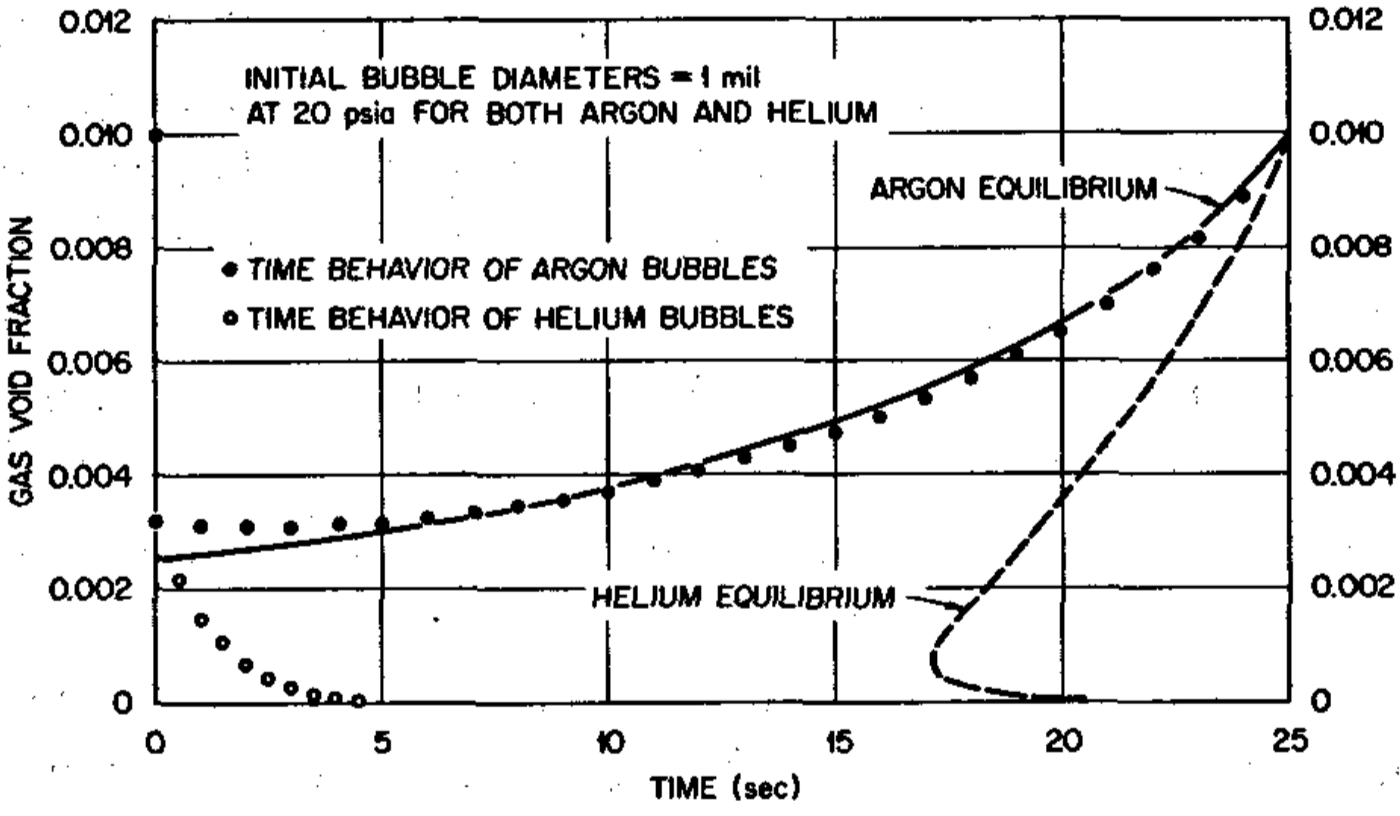
\includegraphics[width=4in]{time_dependent_void.png}\\
  \caption{Time dependent liquid pressure effects on gas void fraction. \cite{steffy1969}}
  \label{fig:time_dependent_void}
\end{figure} 


\newpage

\begin{figure}[ht]
  \centering
  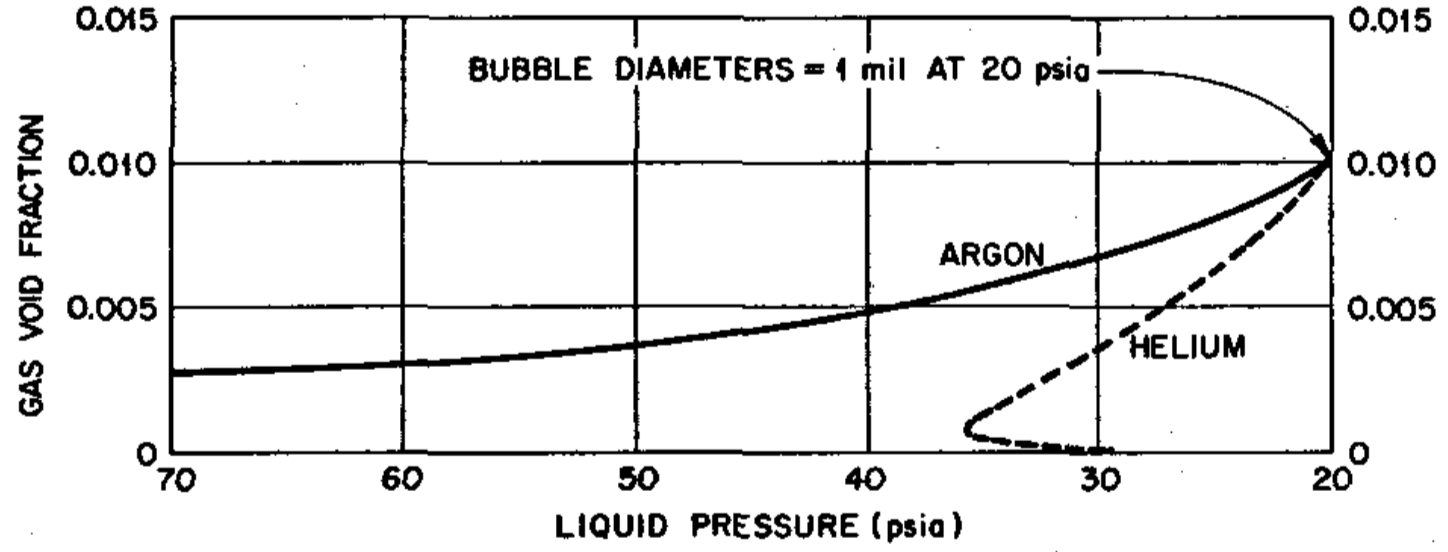
\includegraphics[width=4in]{equilibrium_void.png}\\
  \caption{Equilibrium void fraction vs. liquid pressure. \cite{steffy1969}}
  \label{fig:equ_void}
\end{figure} 



% Mass transport
\subsection{Noble Gas Transport}
As mentioned before, many attempts were made to understand the transport of ${}^{135}$Xe. This section lays out the mathematical models used during the MSRE to transport xenon. The same methods can also be used to model the migration of any volatile gases, assuming that the proper volumetric source terms are taken into account. 

% Mass transfer to moderatior
\subsubsection{Mass Transfer to Moderator}

Depending on reactor design, a moderator might be utilized in slowing down neutrons to induce thermal fissions. This moderator can be directly exposed to the circulating fuel salt, and therefore be subject to mass transfer to its surface along with subsequent diffusion into the material. It is important to note that all species included in the circulating salt are subject to mass transport on and into the moderator. This includes: fission products, fissile material and carrier salt. Three contributing factors that influence this rate include Reynolds number, moderator porosity and diffusion coefficients. As porosity and diffusion coefficient decrease, absorption rates into the moderator decrease. Typically, as Reynolds number increases mass transfer rates increase \cite{watson1962}. 

Pressure changes will not move salt into or out of moderator pores with any appreciable amount, so long as the pores are relatively small. Gas however will, and the rate will vary depending on the nature of the pressure change and the extent of pressure increase over the time interval. The amount of gas in the moderator is a function of the partial pressure in the carrier salt \cite{kedl1972}.

% Mass transfer to circulating voids
\subsubsection{Mass Transfer to Circulating Voids}
During the MSRE sigificant efforts were made to understand ${}^{135}$Xe poisoning. This treatment can be extended to any FP gas. The rate of FP gas migration (atoms per hour) into the circulating bubbles is represented by Equation \ref{eq:migration_rate_xe_MSRE_surface} \cite{houtzeel1967}.

\begin{equation}
    \text{Migration rate to bubbles} = h_{B}A_{B}(C_{S}^{X} - HRTC_{B}^{X})
    \label{eq:migration_rate_xe_MSRE_surface}
\end{equation}

In Equation \ref{eq:migration_rate_xe_MSRE_surface} $C_{s}^{X}$ and $C_{B}^{X}$ are the atomic concentrations of gas X in the salt and bubbles respectively. $A_{B}$ and $h_{B}$ are the interfacial area and mass transfer coefficient. H, R, and T are the Henry's law coefficient, universal gas constant and bubble temperature. Using a model developed in \cite{houtzeel1967} they estimated that small amounts of helium voids would have significant impact on the over all xenon distribution. This is evident from sample calculations indecating that with 0.01 circulating void fraction 98\% of the xenon would be in the bubbles and at 0.001 void, 83\% would be in the bubbles \cite{houtzeel1967}. Using a lumped mass model described in \cite{houtzeel1967}, calculations were preformed to estimate the change in xenon poisoning with mass transfer coefficient, mean bubble diameter and bubble stripping efficiency shown in Figures \ref{fig:MSRE_mass_tranfer}, \ref{fig:MSRE_bubble_size}, \ref{fig:MSRE_bub_strip}.

\vspace{12.7mm} %5mm vertical space

\begin{figure}[ht]
  \centering
  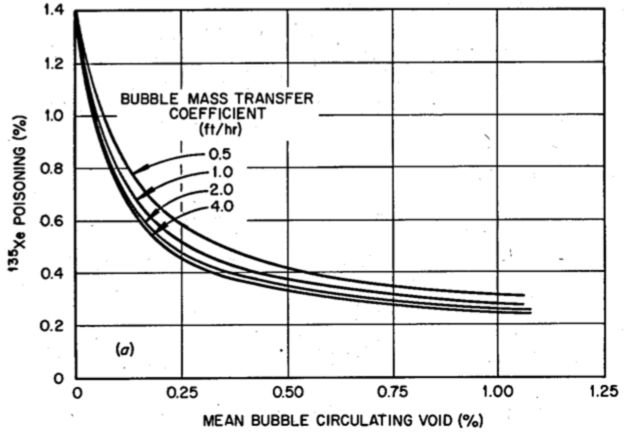
\includegraphics[width=4in]{images/MSRE_mass_transfer_coeff.png}\\
  \caption{Affect of mass transfer coefficient on xenon poisoning}
  \label{fig:MSRE_mass_tranfer}
\end{figure} 

\newpage

\begin{figure}[p]
  \centering
  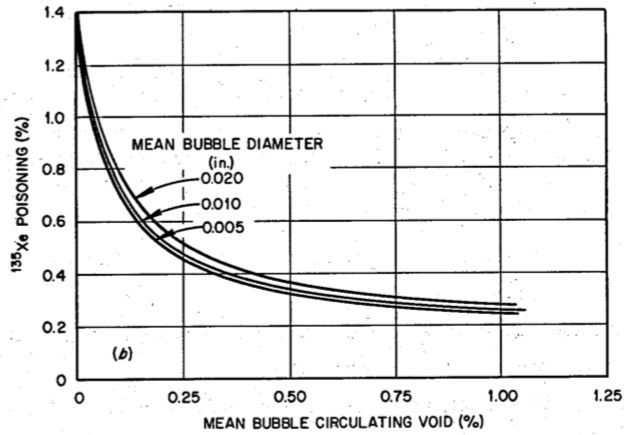
\includegraphics[width=4in]{images/MSRE_mean_bub_dia.png}\\
  \caption{Affect of mean bubbles diameter on xenon poisoning}
  \label{fig:MSRE_bubble_size}
\end{figure} 

\begin{figure}[p]
  \centering
  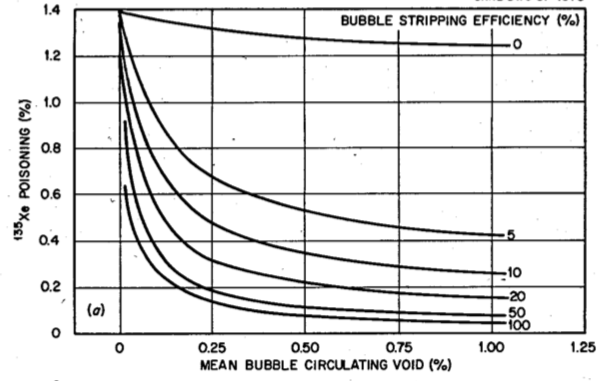
\includegraphics[width=4in]{images/MSRE_bub_stripping.png}\\
  \caption{Affect of bubble stripping efficiency on xenon poisoning}
  \label{fig:MSRE_bub_strip}
\end{figure} 

\FloatBarrier
\newpage

From Figures \ref{fig:MSRE_mass_tranfer} and \ref{fig:MSRE_bubble_size} it was concluded that xenon poisoning is a rather weak function of mass transfer coefficient and bubble diameter. Bubble stripping efficiency has the highest impact on xenon poisoning. These calculations were preformed under the assumption of constant bubble diameter and void fraction. 


% Noble metals
\section{Noble Metals}

The noble metals represent a class of fission products that are reduced by the fuel salt resulting in their existence to be in the solid metallic state.  These reduction reactions are fast and as soon as the noble metals are born they quickly undergo reaction to become neutral metallic nanoparticles \cite{kedl1972}. Reactions of noble metals occur with the fissionable isotope in the fuel salt or components of vessel vie the sample reaction shown in Equation \ref{eq:fp_reduction}. For a structural metal, shown in \ref{eq:metal_reduction}.  

 \begin{equation}
	M^{+n} + nUF_{4} \rightleftharpoons nUF_{3} + MF_{n}
	\label{eq:fp_reduction}
\end{equation}

 \begin{equation}
	M^{+n} + E \rightleftharpoons E^{+n} + M
	\label{eq:metal_reduction}
\end{equation}

In Equation \ref{eq:fp_reduction} fission product $M$ is being reduced by $UF_{4}$ and in Equation \ref{eq:metal_reduction}, $M$ is being reduced by a structural metal $E$. Structural metal $E$ will most likely form an ionic compound with free anions from the carrier salt. 

During MSRE operations, these particles were also found to deposit in the off-gas system and pump bowl. It has also been seen that these noble metals tend to accumulate on vessel and heat exchanger surfaces \cite{kedl1972}. This previously described behavior is due to the fact noble metals have properties much similar to surface active agents which tend to gather around liquid-gas interfaces \cite{kedl1972}. 

% Thermodynamic background
\subsection{Thermodynamic Background}

Oxidation and reduction reactions occur within the molten salt with fission products, fissile material and the metal container. These reactions go on to produce corrosion products and noble metals. A number of fission products may exist as noble metals or as salt seekers and their fate depends upon the redox condition of the salt. 

Redox reactions involve the transfer of electron between reacting species. The species that receives electrons is reduced and the species that donates the electrons is oxidized. The redox condition is often used in referring to a systems propensity to reduce or oxidize a given species. During MSRE operations this term was used when referring to a fission product's tendency to reduce to their metallic state or for the corrosion of container metals \cite{olander2002}. Controlling these reactions (conditioning the salt) is accomplished by controlling the salts tendency to reduce. For either fluoride or chloride based salts, this is done by controlling the potential of diatomic gases anions. 

As mentioned in section \ref{source_terms}, because the reactor operates at such a high temperature, a pseudo equilibrium assumption can be made about the salt. This means that thermodynamic equilibrium is set and reaction equilibrium concentrations can be calculated. Some noble metal reactions almost reach completion while others do not. The ones that do not are known as semi noble metals and their reactivity will be dependent on the redox condition of the salt. In many previous MSR reports, redox condition was a loose term used to describe an elements propensity to undergo redox reactions. Redox condition of the salt is correlated to the chemical potential of the anion either Cl- or F- of the carrier salt \cite{olander2002}.  

For a given reversible chemical reaction,

% General chemical reaction
 \begin{equation}
	v_{A}A + v_{B}B \rightleftharpoons v_{C}C + v_{D}D
	\label{eq:gen_chem_rxn}
\end{equation}

the law of mass action says that,

% Law of mass action
 \begin{equation}
	K_{a} = \prod a_{i}^{v_{i}} = \frac{a_{C}^{v_{C}}a_{D}^{v_{D}}}{a_{A}^{v_{A}}a_{B}^{v_{B}}}
	\label{eq:mass_action}
\end{equation}

therefor at equilibrium and standard state the term on the right-hand side will equal a constant ($K_{a}$) where  is activity and  is stoichiometric coefficient. Chemical activity for the liquid phase can be defined in terms of a substances activity coefficient ($\gamma$) and molar fraction ($x$). 

% activity coefficient
 \begin{equation}
	a_{i} = \gamma_{i}x_{i}
	\label{eq:activity}
\end{equation}

For an ideal solution, the activity coefficient is equal to one and for the gas phase, mole fraction can be replaced with partial pressure. The reaction quotient is related to the Gibbs energy of reaction by, 

 \begin{equation}
	K_{a} = \exp \bigg( \frac{-\Delta G_{rxn}^{o}}{RT} \bigg)
\end{equation}

The change in Gibbs energy with reaction is defined as,

% gibbs reaction
 \begin{equation}
	\Delta G_{rxn}^{o}(T,P) = \Delta G_{f}(products) - \Delta G_{f}(reactants)
	\label{eq:gibbs_rxn}
\end{equation}

The summation of the Gibbs energy of formation for products minus reactants. Gibbs energy is a thermodynamic property which is defined as, 

% gibbs energy
 \begin{equation}
	G = H - TS
	\label{eq:gibbs}
\end{equation}

where $H$ is enthalpy, $T$ is temperature and $S$ is entropy. The change in Gibbs energy is equal to the maximum non-expansion work accompanying a process at constant temperature and pressure. When solutions undergo reactions, the extent is driven toward equilibrium by minimizing the Gibbs energy. This means that for a multicomponent mixture undergoing reactions, the equilibrium species concentrations can be calculated by minimizing the total Gibbs energy of the system. 

In a classical thermodynamic chemical potential is defined as the change in Gibbs energy with number of moles.

% chemical potential
 \begin{equation}
	\Delta \bar{G_{i}^{o}}  = \mu_{i} =  \frac{\partial (nG)}{\partial n_{i}}
	\label{eq:chemical_potential}
\end{equation}

When examining a chemical reaction, the potential of a particular species can be solved for by combining the relations for equilibrium constant and the definition of activity. For example, take reaction shown in equation \ref{eq:gen_chem_rxn}. The law of mass action shows.

 \begin{equation}
	\exp \bigg( \frac{-\Delta G_{rxn}^{o}}{RT} \bigg) = \frac{a_{C}^{v_{C}}a_{D}^{v_{D}}}{a_{A}^{v_{A}}a_{B}^{v_{B}}}
\end{equation}

The chemical potential for reactant A is,

% chemical potential for A
 \begin{equation}
	\Delta \bar{G_{i}^{o}}  = RT\ln(a_{A}) = \frac{1}{v_{A}} \bigg[ RT\ln \bigg( \frac{a_{C}^{v_{C}}a_{D}^{v_{D}}}{a_{B}^{v_{B}}} \bigg) + \Delta G_{rxn} \bigg]
	\label{eq:chemical_potential_A}
\end{equation}

% Noble metal transport
\subsection{Noble Metal Transport}

One of the key requirements for understanding noble metal transport is to first understand their behavior relative to the fluid velocity field. The homogeneous equilibrium model is a simple mixture model which describes the multiphase model as a pseudo single-phase mixture in thermodynamic equilibrium. This model includes assumptions much like the ones which were used to describe two-phase liquid-bubble transport. The primary being that the relative velocities between each phase are zero and each phase is in thermodynamic equilibrium with another. 

Many different surface environments exist in a molten salt loop, which include; moderator, heat exchanger, reactor wall, piping/process equipment and liquid-gas interfaces. Many of these surfaces may not be in thermodynamic equilibrium with the bulk fluid, creating temperature gradients which can affect the amount of noble metal which can deposit. One example of this is in the heat exchanger where bulk fluid temperature is changing as a function of heat exchanger length and fluid velocity. Solubility, which is a function of temperature, begins to change which can lead to a supersaturated state of the liquid solution, leading to increased noble metal deposition. Other processes which can affect surface deposition rates include fluid turbulence, torturous paths and surface area for transfer. 

For noble metal deposition on surfaces, the same convention in which the boundary layer is ignored and a linear convection boundary condition is utilized, equaiton \ref{eq:convection_boundary_condition}. The trick for using this assumption is knowing the mass transfer coefficient  and the surface concentration. Surface concentration can only be assessed if certain assumptions are used. These assumptions deal with the noble metals propensity to stick and stay on the surface and diffuse into the material. A common assumption is to treat the surface material as an infinite sink, making the concentration at the surface zero. This assumption can be used when solving a steady state problem where the surface concentration is unknown. In a time dependent problem, the surface concentration can be assumed to be equal to zero or a given constant. Then for all times greater the surface concentration would be the integral of the flux from zero to the current time or the previous time step. 

An interesting note that comes into play when discussing mass transfer in a saturated system is the affect heterogeneous nucleation has on transfer coefficient. Depending on how the mass transfer coefficient is obtained, nucleation may not be included in the transfer rate. This most then be added to the migration model to obtain a more accurate model. However, if the liquid solution never reaches a point of super saturation, then nucleation does not occur. 

% Noble metal behavior
%\subsection{Noble metal behavior}

%Observations made during the MSRE impart great insight into the general behavior of noble metals in a molten salt environment. During operations, noble metals played a role in many key processes which effected system wide behavior. The behavior includes; deposition on liquid-gas interfaces, plating to container surfaces, and entrapment in the off-gas system. 

%\subsubsection{Liquid-gas interactions}

%As previously noted, noble metals have a tendency to migrate to liquid gas interfaces. This tendency to collect on liquid-gas interfaces follows the same physical model as was surface deposition, however the question remains in finding the surface concentration. During MSRE operation an analytical model was developed for determining migration of noble metals \cite{kedl1972}. From these models, as well as experimental results, it was found that noble metals did not have a tendency to stay on the bubble surface once they became attached. 



